\section{Introduction}\label{i.-introduction}

Urban heat is not distributed uniformly within a city, and the people who live in its hottest
neighbourhoods are frequently those with the least capacity to adapt {[}1{]}, {[}2{]}. This coupling of
hazard and social context is what motivates the development of \emph{heat vulnerability} mapping rather
than heat-hazard mapping alone {[}11{]}, {[}14{]}. Satellite land-surface temperature (LST) has become the
workhorse measurement for such mapping at city scale, because thermal-infrared sensors such as those
aboard Landsat 8 and 9 provide 30 m observations with a validated processing chain {[}1{]}--{[}4{]} and a
long, stable record {[}6{]}.

The decision problem, however, is not merely to produce a map. A municipality must also decide
\emph{where} its measurements are uncertain, \emph{which} places to treat as high priority, and \emph{what} mix of
interventions to buy with a fixed budget, ideally without systematically disadvantaging the
populations already most exposed. Each of these steps has its own methodological literature, and the
most serious errors observed in published urban-heat machine-learning work are methodological rather
than algorithmic. Three recur.

The first is \textbf{optimistic validation}. Random k-fold cross-validation on spatially autocorrelated
data places near neighbours of a test cell in the training set, so reported error understates true
spatial error; this bias has been quantified for large-scale environmental mapping {[}26{]}, {[}27{]}. The
second is \textbf{over-reading of attribution}. Shapley-based explanations describe how a fitted model
uses its inputs; they do not establish that the input causes the outcome {[}28{]}, {[}29{]}. The third is
\textbf{silent conflation of two quantities that look alike}: a percentile computed across spatial pixels
within one cell on one date is not a temporal extreme, and surface temperature is not air
temperature {[}5{]}, {[}11{]}.

Against this background we designed HeatScope to be auditable end to end. Every reported number in
this paper is reproducible from a committed artifact by a fixed script order, and where an artifact
does not support an intended claim we report the narrower claim that it does support rather than
omitting the discrepancy. Section VIII enumerates the cases where this forced a change of framing;
we regard that enumeration as a contribution in its own right, because the affected quantities are
precisely those that decision-makers would otherwise rely on.

The contributions of this work are as follows.

\begin{enumerate}
\def\labelenumi{\arabic{enumi}.}
\tightlist
\item
  A complete 250 m pipeline for Bengaluru producing within-cell upper-tail LST, spectral indices,
  built-form metrics and gridded population, from a single pinned Landsat 8 acquisition through to
  intervention siting, with every intermediate artifact retained.
\item
  A spatially structured evaluation protocol --- five folds over 240 contiguous \textasciitilde2.5 km blocks, with
  a programmatic leakage assertion --- applied not only at final evaluation but to every model and
  every uncertainty estimate in the chain (Section V-B).
\item
  Demonstration that neighbourhood-mean context features measurably improve both accuracy and, more
  importantly, error \emph{balance} across the temperature distribution, reducing hottest-quintile bias
  by 8.08\% (Section VI-C).
\item
  A cross-fitted prediction-interval scheme with reported coverage by temperature quintile, which
  exposes a 7-point coverage deficit in the hottest quintile that a single pooled number conceals
  (Section VI-D).
\item
  An equity-constrained mixed-integer allocation model, with an explicit account of what each
  constraint costs in benefit and of where its inputs come from (Section VI-E).
\item
  A documented negative result: under the implementation's index-based benefit formulation,
  cell-invariant per-intervention effect coefficients cannot influence any ranking (Section VI-E.3).
\end{enumerate}

Section II positions this work. Section III gives the methodology, Section IV the study area and
data, Section V the experimental design, Section VI results, Section VII discussion, Section VIII
limitations, and Section IX concludes.

\section{Related Work}\label{ii.-related-work}

\textbf{Urban heat island remote sensing.} Thermal remote sensing of urban climates {[}5{]} established the
physical basis for retrieving surface temperature and, critically, the distinction between surface and
air temperature that bounds what any LST product can claim. Subsequent reviews catalogue retrieval
methods, scaling problems, and open challenges {[}6{]}, {[}7{]}, and connect mitigation effectiveness to
vulnerability and health outcomes {[}8{]}, {[}9{]}. The magnitude of urban heat islands has been shown to
depend substantially on population and climate rather than urban form alone {[}10{]}, which supports
including demographic covariates alongside spectral ones.

\textbf{Exposure, vulnerability, and human thermal comfort.} Using LST as a proxy for human thermal
exposure is standard practice but carries systematic caveats, most importantly that surface and
near-surface air temperature diverge with time of day, season, and surface moisture {[}5{]}, {[}11{]}.
Exposure time and acclimatization further separate what a thermal index measures from what a person
experiences {[}12{]}. Recent multi-city work on India documents how urbanisation alters heat exposure
risk across Indian cities {[}13{]}.

\textbf{Equity in heat exposure.} Exposure is not merely an environmental quantity but a distributional
one: a detailed analysis of major US cities found systematically disproportionate exposure to urban
heat island intensity {[}14{]}. Normative frameworks for justice criteria in urban climate adaptation
{[}33{]} and operationalised adaptation justice indices {[}34{]} exist but, in the cases we verified, equity
is evaluated on a \emph{finished} hazard map rather than embedded in the allocation decision. The
modifiable-areal-unit sensitivity of environmental-justice findings {[}35{]} further motivates fixing and
justifying an analysis resolution.

\textbf{Spectral indices.} NDVI originates with Rouse et al.~{[}17{]}; the normalised difference moisture index
with Gao {[}15{]}; NDBI with Zha et al.~{[}16{]}. We note in Section VI-B that NDBI and NDMI as defined for
Landsat are algebraic negatives of one another, which is a property of the definitions rather than of
the data.

\textbf{Gridded population and built form.} WorldPop provides 100 m gridded population denominators via
random-forest dasymetric redistribution of census counts {[}18{]}, {[}19{]}, {[}20{]}. Building footprints from
conflated open sources {[}21{]} supply built-form coverage. For Bengaluru specifically, studies have
related LST to urban growth {[}36{]}, land cover by concentric ring {[}37{]}, and the controlling
biophysical factors {[}38{]}; tropical Indian-city work supports the vegetation and urbanisation feature
set used here {[}39{]}.

\textbf{Modelling method.} Gradient-boosted decision trees {[}22{]} and their scalable variants {[}23{]} are the
workhorses of tabular environmental prediction; extremely randomised trees {[}24{]} and random forests
{[}25{]} provide standard tree-ensemble baselines.

\textbf{Spatially structured validation.} Roberts et al.~{[}26{]} provide the definitive treatment of
cross-validation under spatial, temporal, hierarchical and phylogenetic structure. Ploton et al.
{[}27{]} quantify the resulting optimism for spatial prediction problems.

\textbf{Explainability.} TreeSHAP {[}28{]} and the original Shapley formulation {[}29{]} provide exact additive
attributions for tree ensembles, which is what permits attribution to be propagated into downstream
scenario weights rather than merely displayed.

\textbf{Predictive uncertainty.} Split conformal prediction {[}30{]} and its exposition {[}31{]} define the
conditions under which a nominal 95\% interval actually carries 95\% coverage. We use these as the
benchmark our intervals are measured against, and we state explicitly where they fall short.

\textbf{Sensitivity analysis.} Design-based Monte Carlo practice and its reporting requirements are set
out by Saltelli et al.~{[}32{]}.

\textbf{Optimisation.} The allocation stage solves a mixed-integer program through the HiGHS solver
{[}40{]}, {[}41{]}. We were unable to verify a peer-reviewed formulation that allocates urban heat
mitigation under budget and equity constraints, and we note this gap rather than cite a loosely
related study.

\section{Methodology}\label{iii.-methodology}

\subsection{Overview}\label{a.-overview}

Fig. 1 gives the pipeline as implemented. Four data layers --- Landsat Collection 2 Level-2 surface
reflectance and surface temperature, conflated building footprints, and gridded population --- are
reduced to a common 250 m grid. Spectral indices and zonal statistics form a feature table. Neighbour
context features are derived from that table. Models are trained and assessed under block-grouped
spatial cross-validation; attribution is computed and propagated into a priority score and
intervention benefit weights; a mixed-integer program allocates interventions; a Monte Carlo
analysis perturbs the scenario parameters.

\begin{figure*}[!t]
\centering
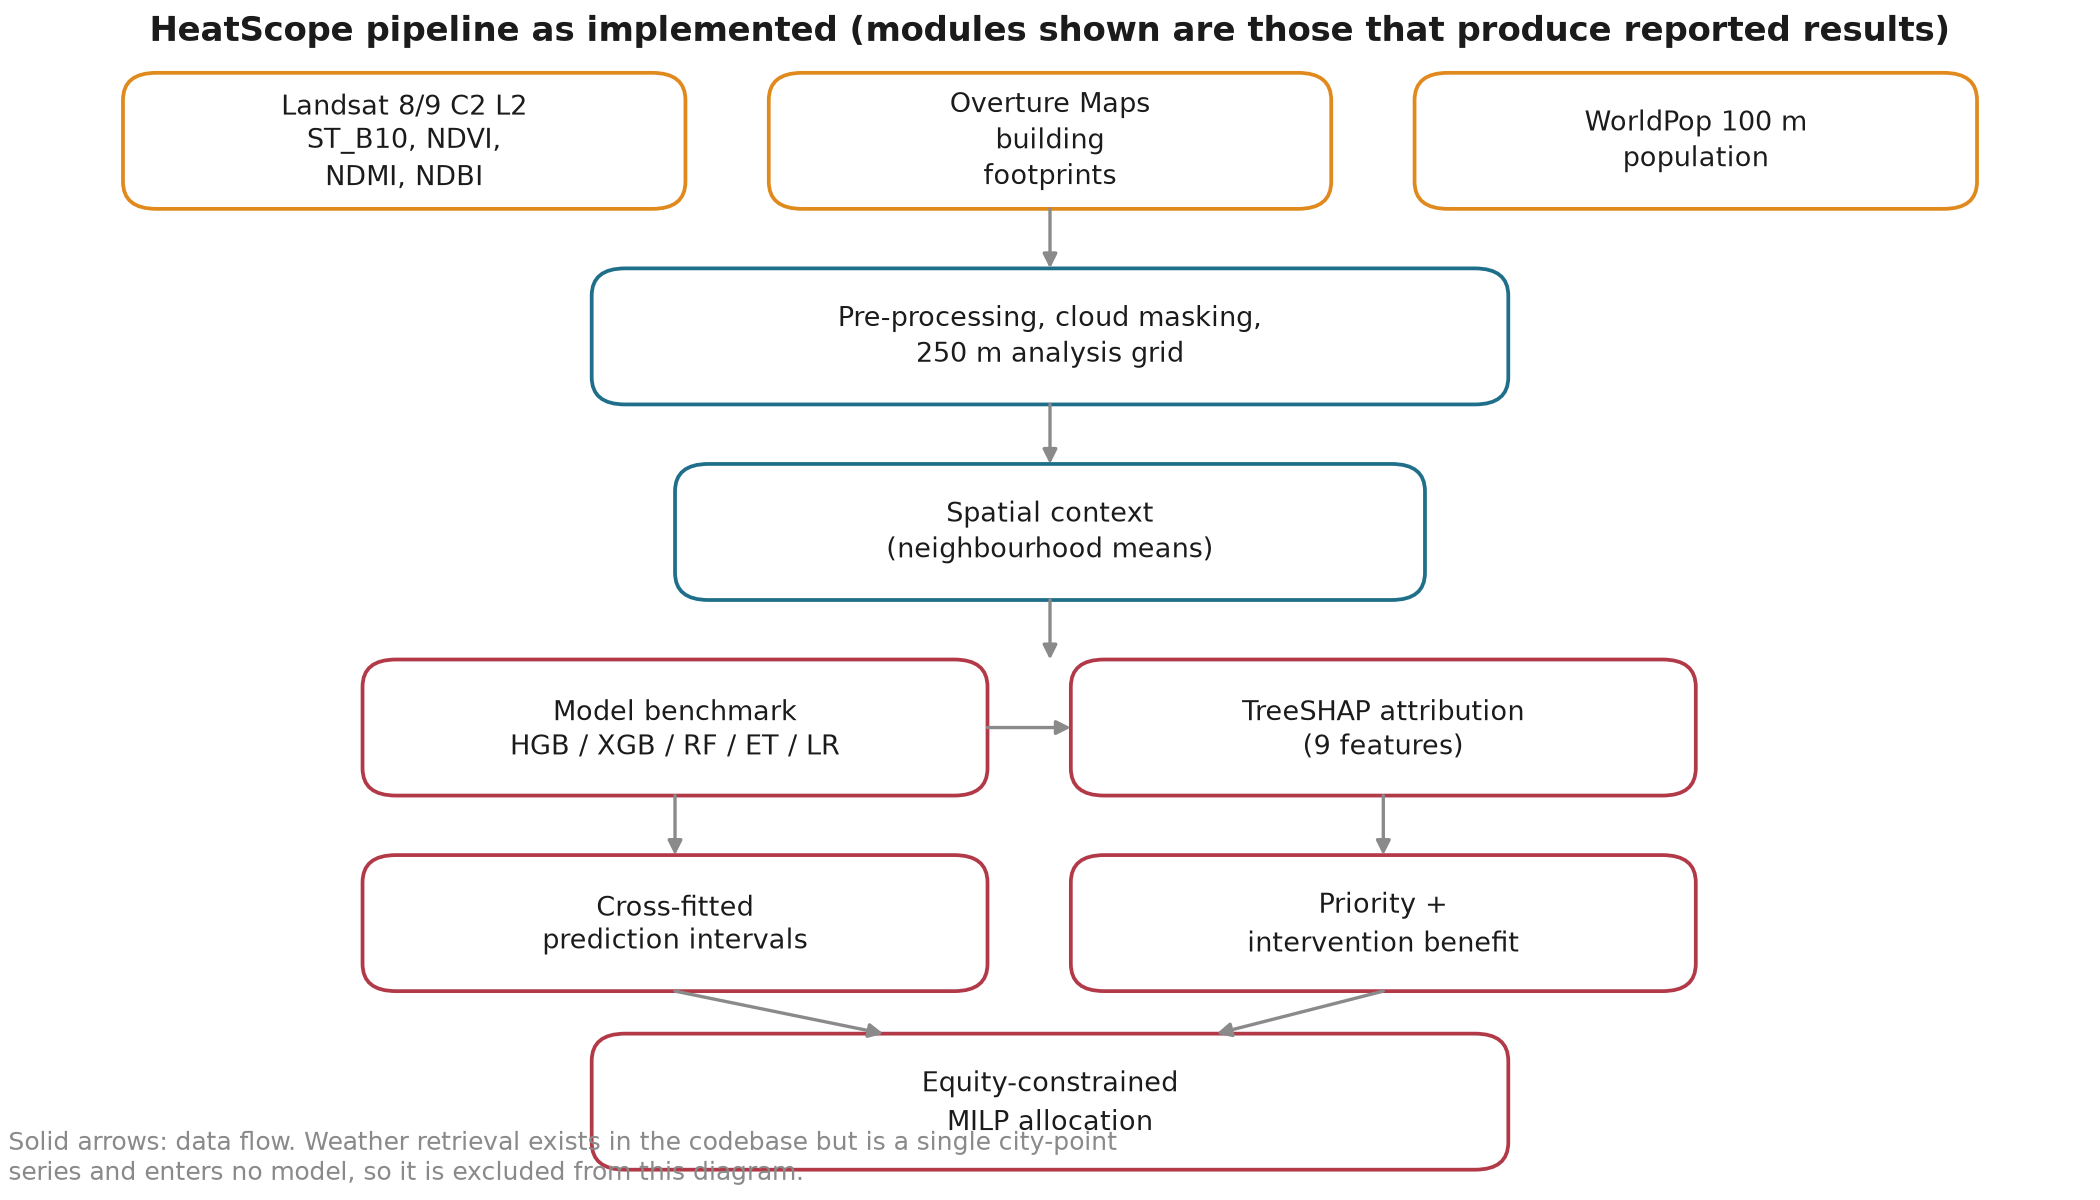
\includegraphics[width=\linewidth]{figures/fig1_architecture.png}
\caption{HeatScope as implemented. Modules shown are those that produce reported results. Weather retrieval exists in the codebase but yields a single city-point series and enters no model, so it is excluded.}
\label{fig:1}
\end{figure*}


\subsection{Pre-processing and grid construction}\label{b.-pre-processing-and-grid-construction}

A single Landsat 8 Collection 2 Level-2 scene is retrieved from STAC: collection \texttt{landsat-c2-l2},
path 144, row 051, acquisition 2026-04-01 05:10:29 UTC, reported cloud cover 0.23\%
(\texttt{LC08\_L2SP\_144051\_20260401\_02\_T1}). Assets \texttt{red}, \texttt{nir08}, \texttt{swir16}, \texttt{lwir11} and \texttt{qa\_pixel} are
used. Radiometric scaling follows the Collection 2 conventions {[}1{]}, {[}2{]}: surface reflectance is
computed as \(\rho = 0.0000275 \times DN - 0.2\), and land-surface temperature as
\(T_{C} = 0.00341802 \times DN + 149.0 - 273.15\).

Quality screening is applied per pixel. Pixels are masked where the \texttt{QA\_PIXEL} band flags fill,
dilated cloud, cirrus, cloud, cloud shadow, or snow; where any band's digital number is
non-positive; where scaled reflectance falls outside \([0, 1]\); where LST falls outside
\([-50, 80]\,^{\circ}\mathrm{C}\); or where any computed index falls outside \([-1, 1]\). The resulting
masked scene contains 39,624,101 valid 30 m pixels over a 7541 \texttimes{} 7701 window in UTM zone 43N
(EPSG:32643).

Three normalised indices are computed per pixel:

\[\mathrm{NDVI} = \frac{NIR - RED}{NIR + RED} \tag{1}\]

\[\mathrm{NDBI} = \frac{SWIR - NIR}{SWIR + NIR} \tag{2}\]

\[\mathrm{NDMI} = \frac{NIR - SWIR}{NIR + SWIR} \tag{3}\]

The analysis grid is a regular 250 m lattice in EPSG:32643 whose extent is derived from the
temperature raster, clipped to the study-region polygon, and renumbered. It contains 21,845 cells
totalling 1,348.25 km². Because cells are clipped to the study-region polygon, boundary cells have
reduced area; 30 cells have an area below 25\% of nominal, the smallest being 10.54 m². These are
retained but flagged, and Section VIII discusses their influence.

\subsection{Feature construction}\label{c.-feature-construction}

Eleven predictors are used in the base model. Spectral features are the per-cell mean and median
of NDVI, NDBI and NDMI, six statistics in total. Demographic and built-form features are population
count, population density, building count, building area and building coverage percentage, five
more. The within-cell 95th percentile of LST is the target and is never supplied to the model.

Two implementation properties are consequential and are reported as findings rather than hidden.
First, the denominators in (2) and (3) are the same expression with the numerator sign reversed, so
\(\mathrm{NDBI} \equiv -\mathrm{NDMI}\) exactly for every pixel. We verified this numerically:
\(\max|\mathrm{NDBI} + \mathrm{NDMI}| = 0.0\) over all 39,624,101 valid pixels, and the Spearman
correlation between the two per-cell means is exactly \(-1.0000\). The eleven-feature set therefore
contains one redundant pair, and the reduced five-feature set used in the ablation removes NDBI.
Second, population is aggregated from the 100 m population raster by centre-in-cell selection with
no proportional-area weighting, so cells straddling raster edges can be miscounted by up to one raster
pixel.

\subsection{Neighbourhood context features}\label{d.-neighbourhood-context-features}

For each of four features --- NDVI, NDMI, population density and building coverage --- the mean over
queen-contiguous neighbours is computed, excluding the focal cell itself. Queen adjacency is
established by a spatial-index candidate query followed by an exact touches-or-intersects test.
Excluding the focal cell guarantees that no feature value can enter the feature vector that describes
it. Four context columns are carried forward; local-contrast and neighbourhood-standard-deviation
columns are computed by the same routine but are not consumed downstream.

\subsection{Heat vulnerability layer}\label{e.-heat-vulnerability-layer}

A composite index is computed to support descriptive mapping and, more importantly, to supply the
structural-vulnerability term used downstream. Each component is normalised by clipping to its 1st
and 99th percentiles and rescaling to \([0, 1]\). An exposure score combines normalised mean LST (0.50),
normalised p95 LST (0.30) and normalised mean NDBI (0.20). A capacity score combines normalised mean
NDVI (0.45), normalised mean NDMI (0.35) and a normalised built-form deficit (0.20). A sensitivity
score is the normalised log population density. The index is the product
\(\mathrm{exposure} \times \mathrm{sensitivity} \times (1 - \mathrm{capacity})\), rescaled, ranked, and
cut into quintile categories. These weights are expert-elicited and are not validated; Section VIII
states the consequences.

\subsection{Attribution}\label{f.-attribution}

TreeSHAP {[}28{]}, {[}29{]} is computed for the nine-feature context model over 5,000 cells stratified by
target quantile. Because the explainer uses interventional perturbation estimated from a 100-row
background sample, additivity is approximate; the measured discrepancy between
\(\mathrm{base} + \sum_j \phi_j\) and the model prediction is reported in Section VI-C. Attribution
values are used twice: as a diagnostic of which predictors the model relies on, and as input to the
priority construction described next.

\subsection{Priority and intervention benefit}\label{g.-priority-and-intervention-benefit}

The priority construction is deliberately retrospective-free. Exposure enters only through
out-of-fold \emph{predicted} LST; the observed temperature is never used. A risk term combines the
prediction with an uncertainty half-width, and a structural-vulnerability term combines normalised
log population density with the built-form capacity score. The operational priority is a weighted
blend of the normalised risk term and the structural-vulnerability term, with cells in the top 30\% of
structural vulnerability flagged as equity-priority cells.

For each cell and each of four intervention types --- urban tree, shade structure, cool roof and
cooling centre --- an \emph{opportunity} term expresses physical or demographic suitability, computed
exclusively from remotely sensed and demographic quantities so that the benefit model does not
circularly consume the target. A need term combines the risk and structural-vulnerability terms. The
per-cell benefit for intervention type \(t\) is

\[\begin{aligned}\mathrm{benefit}_{i,t} &= \mathrm{need}_i \times \mathrm{opportunity}_{i,t} \\ &\quad \times \mathrm{effect}_t \times \mathrm{populationFactor}_i \end{aligned} \tag{4}\]

with scenario parameters \(\mathrm{effect}_t\) and unit costs given in Table V. One property of (4)
deserves emphasis because it constrains what can be claimed: \(\mathrm{effect}_t\) is a
\emph{cell-invariant constant} per intervention type, so it multiplies every cell identically and
therefore cannot alter any per-cell ranking. Its only influence is through the cost--benefit
trade-off inside the allocation model. Any statement that one intervention is preferable to another
\emph{because of its effect coefficient} would be circular; Section VI-E.3 confirms this empirically.

Eligibility gates restrict which cells each intervention may serve. Each gate is a conjunction of
in-sample median or quartile thresholds on NDVI, NDMI, building coverage, population density, risk
and structural vulnerability. Section VI-F discusses what this implies for the resulting eligibility
rate.

\subsection{Equity-constrained allocation}\label{h.-equity-constrained-allocation}

Let \(x_{i,t} \in \{0,1\}\) indicate that intervention type \(t\) is assigned to cell \(i\). The
allocation model maximises total benefit subject to a per-cell single-intervention constraint, a
budget constraint, per-type capacity limits, and an equity floor:

\[\max \sum_i \sum_t \mathrm{benefit}_{i,t} \, x_{i,t} \tag{5}\]

\[\text{s.t.}\quad \sum_t x_{i,t} \leq 1 \ \forall i \tag{6}\]

\[\sum_i \sum_t \mathrm{cost}_t \, x_{i,t} \leq B \tag{7}\]

\[\sum_t x_{i,t} \leq C_t \quad \forall t \tag{8}\]

\[(1 - \alpha) \sum_{i \in \mathcal{E}} \mathrm{benefit}_{i,t} x_{i,t} - \alpha \sum_{i \notin \mathcal{E}} \mathrm{benefit}_{i,t} x_{i,t} \geq 0 \tag{9}\]

where \(\mathcal{E}\) is the equity-priority set and constraint (9) is equivalent to a floor \(\alpha\) on
the share of benefit accruing to \(\mathcal{E}\). Solutions are obtained with HiGHS {[}40{]}, {[}41{]} via
\texttt{scipy.optimize.milp} with a relative MIP gap of \(10^{-4}\).

Two configurations are reported. In the \textbf{capacity-bound} configuration the budget is
\(n_{cells} \bar{c} f\) with \(\bar{c}\) the mean unit cost and \(f = 0.5\); capacities bind and the budget
does not. In the \textbf{budget-bound} configuration the budget is \(f \sum_t c_t C_t\) with
\(f \in \{0.25, 0.5, 0.75, 1.0\}\); the budget binds at utilisation 0.9999--1.0000 and capacities are
slack. Section VI-E reports both and states which constraint is active in each.

\subsection{Monte Carlo sensitivity}\label{i.-monte-carlo-sensitivity}

Cost and effect coefficients are perturbed by uniform multiplicative factors on \([0.7, 1.3]\) and
capacities by factors on \([0.8, 1.2]\), with capacity ceilings rounded to integers and floored at one.
500 runs are executed: 100 selection-pipeline runs and 50 equity-pipeline runs, each evaluated across
multiple budget and equity settings. The random seed is fixed at 42.

\section{Study Area and Data}\label{iv.-study-area-and-data}

The study region is a 0.33\textdegree{} \texttimes{} 0.34\textdegree{} bounding box (12.82--13.16\textdegree{} N, 77.45--77.78\textdegree{} E) enclosing the
Bengaluru metropolitan area in the Indian state of Karnataka, analysed on a 250 m grid of 21,845
cells covering 1,348.25 km². Of these, 21,815 carry a valid temperature target. The region contains
a gridded population of 7,458,314 persons, a mean density of 5,533 persons per km\(^2\).

Bengaluru is an appropriate case for three reasons. It is among the larger and faster-growing Indian
metropolitan areas; LST--urban-growth relationships there are already documented {[}36{]}, {[}37{]} and the
controlling biophysical factors identified {[}38{]}; and the tropical semi-arid setting means that
vegetation and moisture contrasts are strong, which is the regime in which the vegetation and
moisture indices carry the most signal.

\begin{table}[!t]
\caption{Data sources and characteristics.}
\label{tab:1}
\centering
\footnotesize
\begin{tabular}{@{}
>{\raggedright\arraybackslash}p{(\linewidth - 6\tabcolsep) * \real{0.2500}}
  >{\raggedright\arraybackslash}p{(\linewidth - 6\tabcolsep) * \real{0.2500}}
  >{\raggedright\arraybackslash}p{(\linewidth - 6\tabcolsep) * \real{0.2500}}
  >{\raggedright\arraybackslash}p{(\linewidth - 6\tabcolsep) * \real{0.2500}}@{}}
\toprule\noalign{}
\begin{minipage}[b]{\linewidth}\raggedright
Layer
\end{minipage} & \begin{minipage}[b]{\linewidth}\raggedright
Source
\end{minipage} & \begin{minipage}[b]{\linewidth}\raggedright
Native resolution
\end{minipage} & \begin{minipage}[b]{\linewidth}\raggedright
Role
\end{minipage} \\
\midrule\noalign{}
Surface temperature, surface reflectance & Landsat 8 C2 L2, path 144 / row 051, 2026-04-01, cloud 0.23\% & 30 m & Target and spectral predictors \\
Building footprints & Overture Maps Buildings theme, snapshot 2026-08-13, quadkey 123303312, ODbL & Vector & Count, area, coverage \\
Population & WorldPop 100 m gridded denominators {[}20{]} & \textasciitilde100 m & Count, density \\
Derived grid & This work & 250 m & Analysis unit \\
\end{tabular}
\end{table}


Note that the study region is a bounding box rather than an administrative boundary, and that the
building layer is a single quadkey tile of a global conflation product rather than a complete
extract.

\begin{figure*}[!t]
\centering
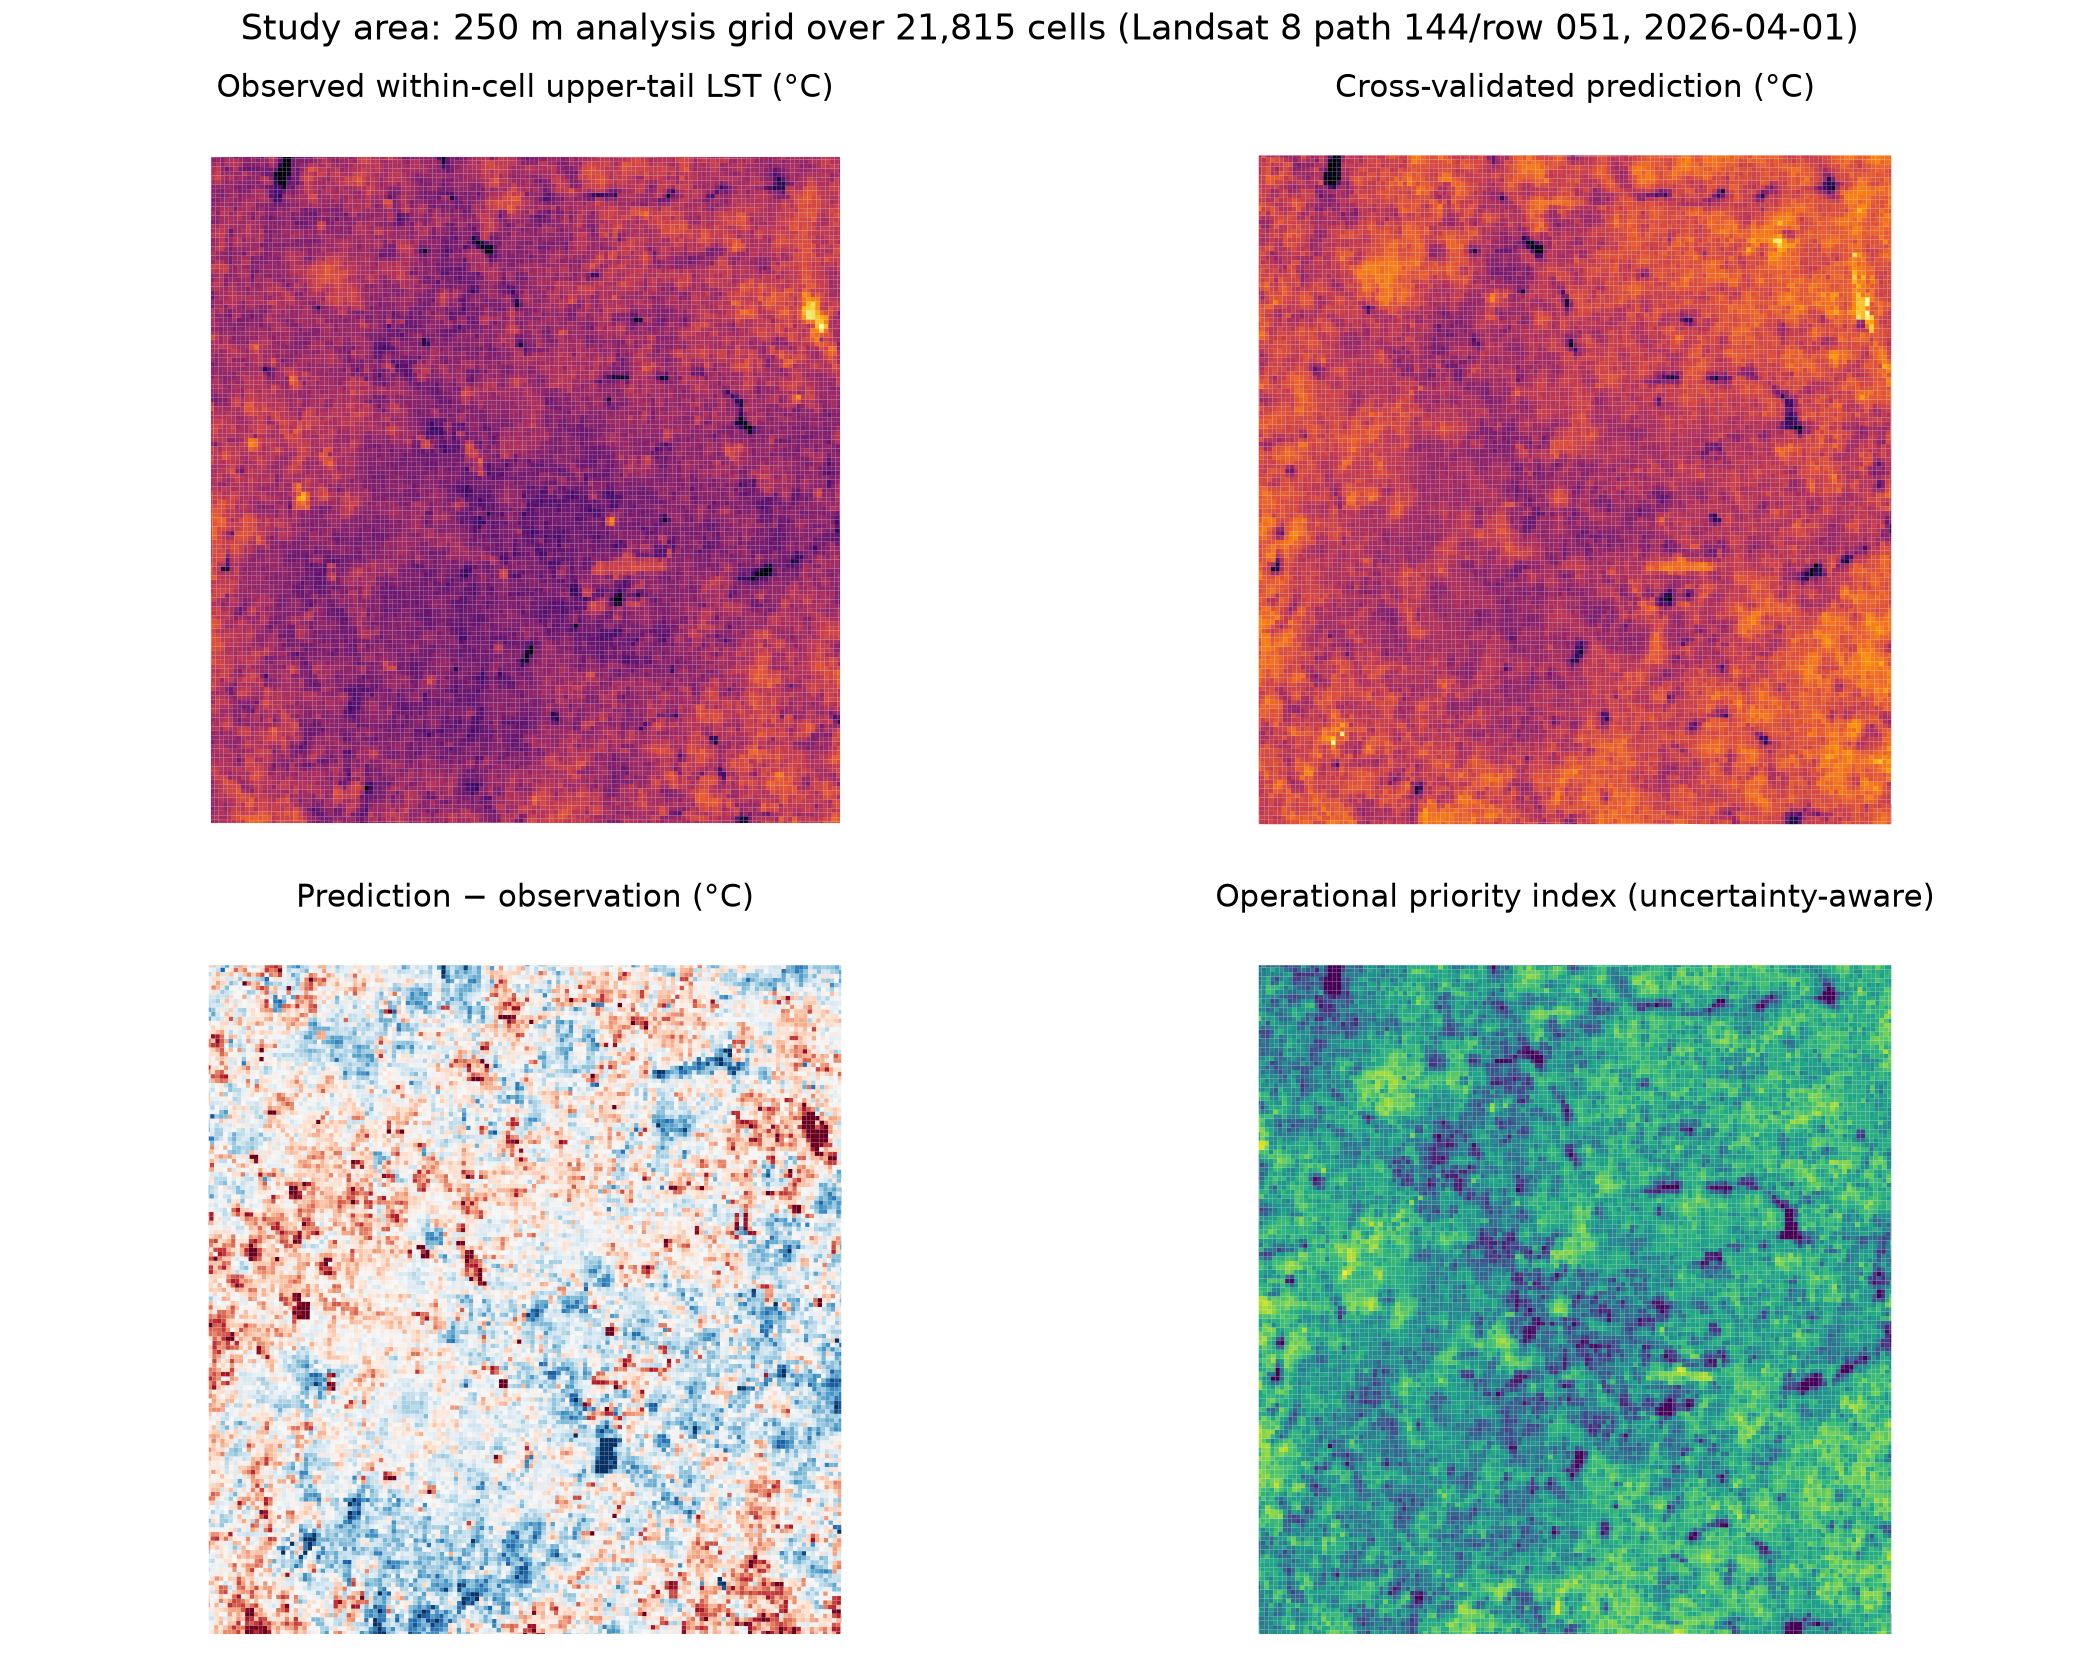
\includegraphics[width=\linewidth]{figures/fig2_study_area.png}
\caption{Observed within-cell upper-tail LST, cross-validated prediction, prediction residual, and the operational priority index. The systematic warm residual over the urban core corresponds to the positive hottest-quintile bias quantified in Section VI-C.}
\label{fig:2}
\end{figure*}


\section{Experimental Design}\label{v.-experimental-design}

\subsection{Predictors and models}\label{a.-predictors-and-models}

Five estimators are benchmarked under identical folds and identical predictors:
HistGradientBoostingRegressor (300 iterations, learning rate 0.05, 31 leaves, L2 1.0),
XGBRegressor (500 estimators, depth 6, learning rate 0.05, subsample 0.8, column subsample 0.8),
RandomForestRegressor (300 trees, \(\sqrt{p}\) features, minimum leaf 2), ExtraTreesRegressor (300
trees, all features, minimum leaf 2), and a standardised linear regression. All stochastic components
use seed 42.

Three feature sets are compared. The \textbf{11-feature} base set is the full predictor list above. The
\textbf{5-feature} reduced set drops NDVI median, both NDBI statistics, NDMI median, population count and
building area, retaining NDVI mean, NDMI mean, population density, building coverage percentage and
building count. The \textbf{9-feature context} set is that reduced set plus the four neighbourhood means,
and it is the model whose results the paper reports as primary.

\subsection{Spatially structured cross-validation}\label{b.-spatially-structured-cross-validation}

Cells are assigned to 240 contiguous blocks of approximately 2.5 km using a row--column block
identifier, giving exactly 48 blocks per fold. Five-fold grouped cross-validation holds out whole
blocks, so that no training cell is spatially adjacent to a test cell through block membership. The
implementation asserts disjoint block sets and raises an error otherwise. Training sets contain
17,447--17,455 cells and test sets 4,360--4,368 cells.

Because fold-to-fold variation is substantial relative to the differences between models, all
performance figures are reported as mean \textpm{} standard deviation over the five folds. The hottest-
quintile stratification is cut on the pooled target before cross-validation and is used only for
reporting, never as a feature; pooled quintile statistics are therefore reported, not per-fold
quintile statistics.

\subsection{Uncertainty evaluation}\label{c.-uncertainty-evaluation}

For each held-out fold, the 90th and 95th percentiles of absolute residual are computed from the
\emph{other} four folds and used as symmetric half-widths. This is fold-wise cross-fitting. We do \textbf{not}
claim formal conformal validity: the quantiles are estimated by linear interpolation rather than by
the conformal index \(\lceil (n+1)(1 - \alpha) \rceil\), and the calibration residuals for a given fold
originate from models trained on folds that include it. Section VI-D reports what this scheme
actually achieves.

\subsection{Reproducibility protocol}\label{d.-reproducibility-protocol}

Every module was re-executed from the committed code and compared against the pre-existing
artifacts. Base-model fold metrics agreed to within \(4.4 \times 10^{-16}\); context-model metrics
agreed exactly; the SHAP importance table was byte-identical; both interval schemes reproduced their
reported coverage and width exactly. Separately, the predictions stored in the operational-priority
artifact were compared against the regenerated model output across all 21,815 cells, giving a
maximum absolute difference of exactly 0.0. Section VIII records the two reproducibility
limitations that this protocol exposed.

\section{Results}\label{vi.-results}

\subsection{Model comparison}\label{a.-model-comparison}

\begin{table*}[!t]
\caption{Out-of-fold performance, 11-feature set, five block-grouped folds (mean \textpm{} SD).}
\label{tab:2}
\centering
\footnotesize
\begin{tabular}{@{}
>{\raggedright\arraybackslash}p{(\linewidth - 6\tabcolsep) * \real{0.2500}}
  >{\raggedright\arraybackslash}p{(\linewidth - 6\tabcolsep) * \real{0.2500}}
  >{\raggedright\arraybackslash}p{(\linewidth - 6\tabcolsep) * \real{0.2500}}
  >{\raggedright\arraybackslash}p{(\linewidth - 6\tabcolsep) * \real{0.2500}}@{}}
\toprule\noalign{}
\begin{minipage}[b]{\linewidth}\raggedright
Model
\end{minipage} & \begin{minipage}[b]{\linewidth}\raggedright
MAE (\textdegree{}C)
\end{minipage} & \begin{minipage}[b]{\linewidth}\raggedright
RMSE (\textdegree{}C)
\end{minipage} & \begin{minipage}[b]{\linewidth}\raggedright
R²
\end{minipage} \\
\midrule\noalign{}
HistGradientBoosting & \textbf{1.213 \textpm{} 0.051} & \textbf{1.591 \textpm{} 0.070} & \textbf{0.636 \textpm{} 0.043} \\
XGBoost & 1.215 \textpm{} 0.047 & 1.595 \textpm{} 0.069 & 0.634 \textpm{} 0.042 \\
RandomForest & 1.218 \textpm{} 0.051 & 1.596 \textpm{} 0.074 & 0.633 \textpm{} 0.045 \\
ExtraTrees & 1.226 \textpm{} 0.054 & 1.607 \textpm{} 0.076 & 0.628 \textpm{} 0.046 \\
LinearRegression & 1.290 \textpm{} 0.068 & 1.698 \textpm{} 0.089 & 0.585 \textpm{} 0.054 \\
\end{tabular}
\end{table*}


Gradient boosting gives the best mean performance on all three metrics. The margin over the runner-up
is 0.002 \textdegree{}C in MAE, which is more than an order of magnitude smaller than the fold-to-fold standard
deviation of approximately 0.05 \textdegree{}C. We therefore describe the tree ensembles as performing
comparably, and note that this study is not powered to separate them. The linear model is
approximately 6\% worse in MAE, which is the one comparison that survives the fold variability.

\begin{figure*}[!t]
\centering
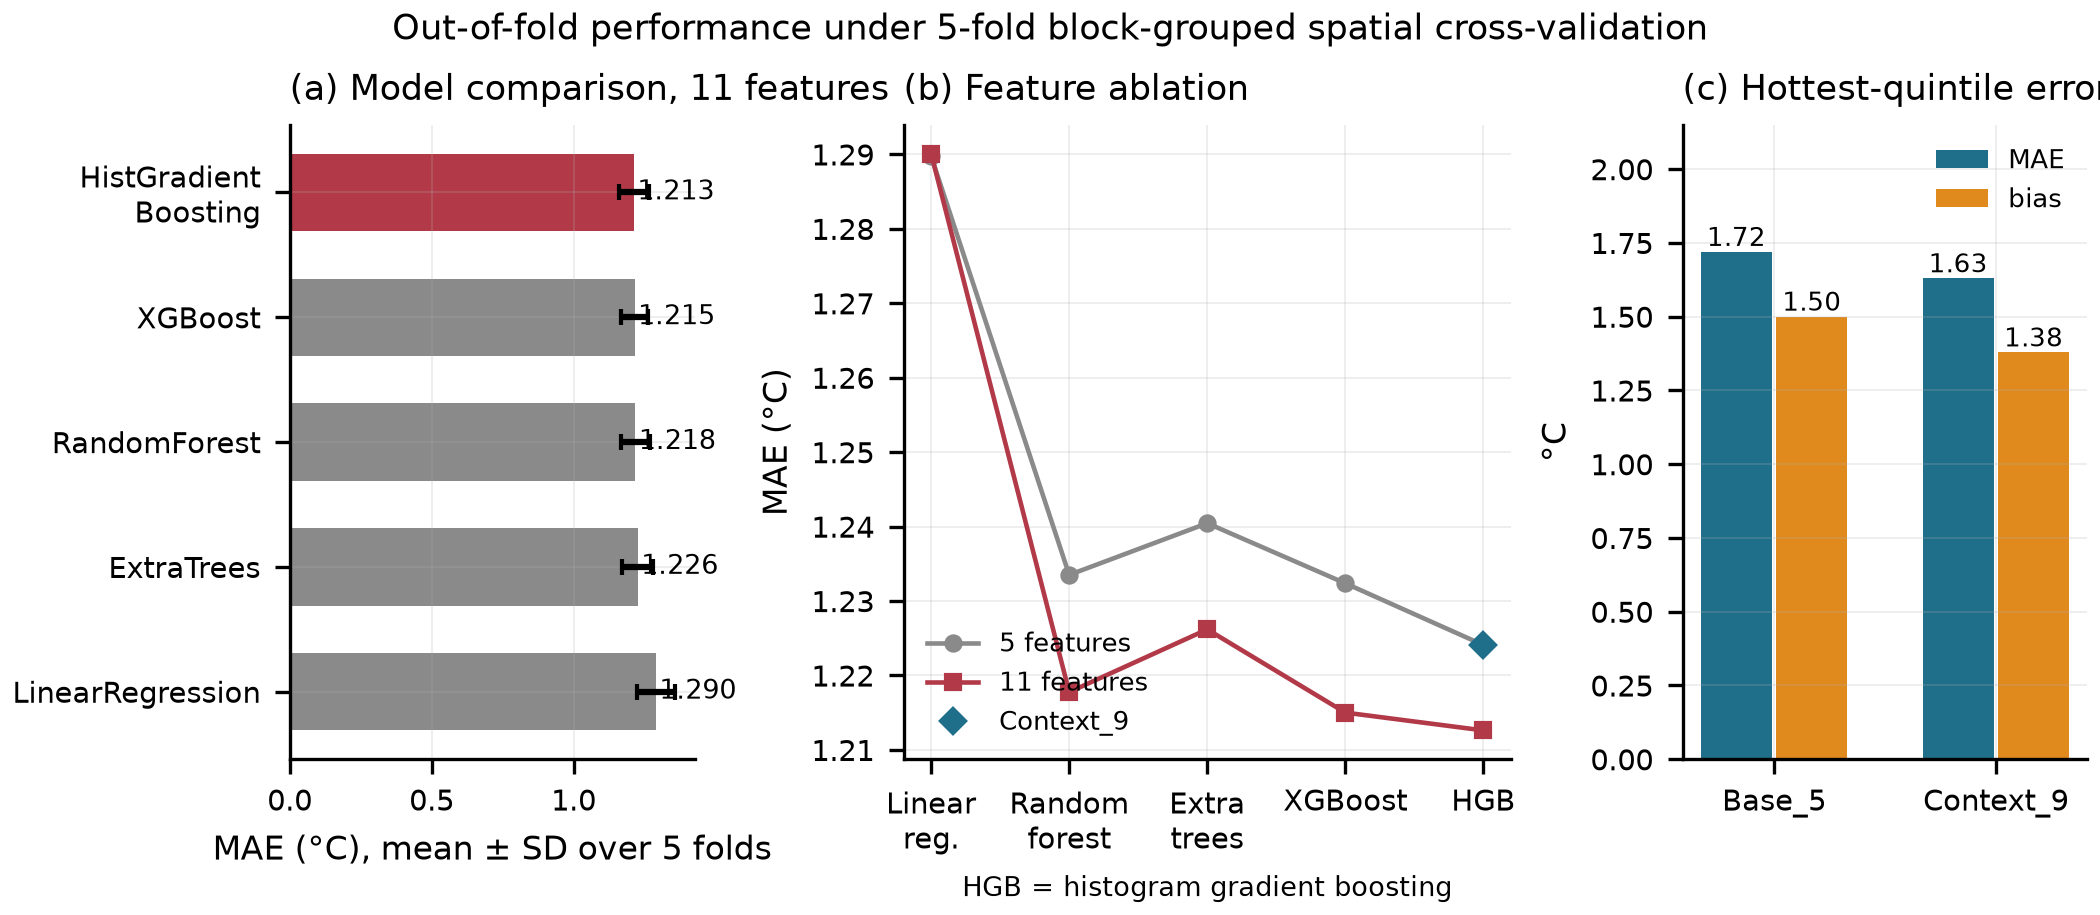
\includegraphics[width=\linewidth]{figures/fig3_models.png}
\caption{Model panels: (a) model comparison with fold dispersion, (b) feature ablation, and (c) hottest-quintile error and bias before and after adding neighbourhood context.}
\label{fig:3}
\end{figure*}


\subsection{Feature audit and index redundancy}\label{b.-feature-audit-and-index-redundancy}

The per-cell means of NDBI and NDMI correlate at exactly \(-1.0000\), and their univariate Spearman
association with the target is identical at 0.7416 and \(-0.7416\) respectively. This is an algebraic
identity of definitions (1)--(3), not an empirical finding, and it means the apparent contribution of
two indices in the 11-feature base set is one. The remaining redundancy structure is milder but non-trivial: NDVI
mean and median correlate at 0.9793, building coverage and building area at 0.9990, and population
count and density at 0.9985.

\subsection{Neighbourhood context and error balance}\label{c.-neighbourhood-context-and-error-balance}

Adding four neighbourhood-mean features improves every reported metric, and improves the \emph{hottest
cells} more than the average cell.

\begin{table}[!t]
\caption{Feature-set ablation (five block-grouped folds).}
\label{tab:3}
\centering
\footnotesize
\begin{tabular}{@{}
>{\raggedright\arraybackslash}p{(\linewidth - 10\tabcolsep) * \real{0.1667}}
  >{\raggedright\arraybackslash}p{(\linewidth - 10\tabcolsep) * \real{0.1667}}
  >{\raggedright\arraybackslash}p{(\linewidth - 10\tabcolsep) * \real{0.1667}}
  >{\raggedright\arraybackslash}p{(\linewidth - 10\tabcolsep) * \real{0.1667}}
  >{\raggedright\arraybackslash}p{(\linewidth - 10\tabcolsep) * \real{0.1667}}
  >{\raggedright\arraybackslash}p{(\linewidth - 10\tabcolsep) * \real{0.1667}}@{}}
\toprule\noalign{}
\begin{minipage}[b]{\linewidth}\raggedright
Feature set
\end{minipage} & \begin{minipage}[b]{\linewidth}\raggedright
MAE (\textdegree{}C)
\end{minipage} & \begin{minipage}[b]{\linewidth}\raggedright
RMSE (\textdegree{}C)
\end{minipage} & \begin{minipage}[b]{\linewidth}\raggedright
R²
\end{minipage} & \begin{minipage}[b]{\linewidth}\raggedright
Q5 MAE (\textdegree{}C)
\end{minipage} & \begin{minipage}[b]{\linewidth}\raggedright
Q5 bias (\textdegree{}C)
\end{minipage} \\
\midrule\noalign{}
Reduced (5) & 1.2241 & 1.6060 & 0.6286 & 1.7198 & +1.5005 \\
Context (9) & \textbf{1.1738} & \textbf{1.5478} & \textbf{0.6548} & \textbf{1.6305} & \textbf{+1.3792} \\
Change & \textminus{}4.11\% & \textminus{}3.62\% & +0.026 & \textminus{}5.19\% & \textminus{}8.08\% \\
\end{tabular}
\end{table}


The 3.62\% RMSE reduction and +0.026 R² gain are modest but consistent. The more informative result
is the bias column. In the hottest quintile the mean observed value exceeds the mean prediction by
1.38 \textdegree{}C --- a systematic under-prediction of precisely the cells a heat-adaptation programme would target
first. Neighbourhood context reduces this bias by 8.08\%, which is directionally encouraging but does
not eliminate it. We regard the residual bias, not the headline MAE, as the principal modelling
finding of this study.

Attribution for the context model (Fig. 4) shows that the four neighbourhood features jointly account
for \textbf{45.42\%} of total attribution --- more than the four focal features combined (54.58\%). NDMI alone,
summing focal and neighbourhood contributions, accounts for 49.38\%. This is the quantitative basis for
propagating attribution into the downstream benefit model rather than presenting it only as a
diagnostic.

\begin{figure*}[!t]
\centering
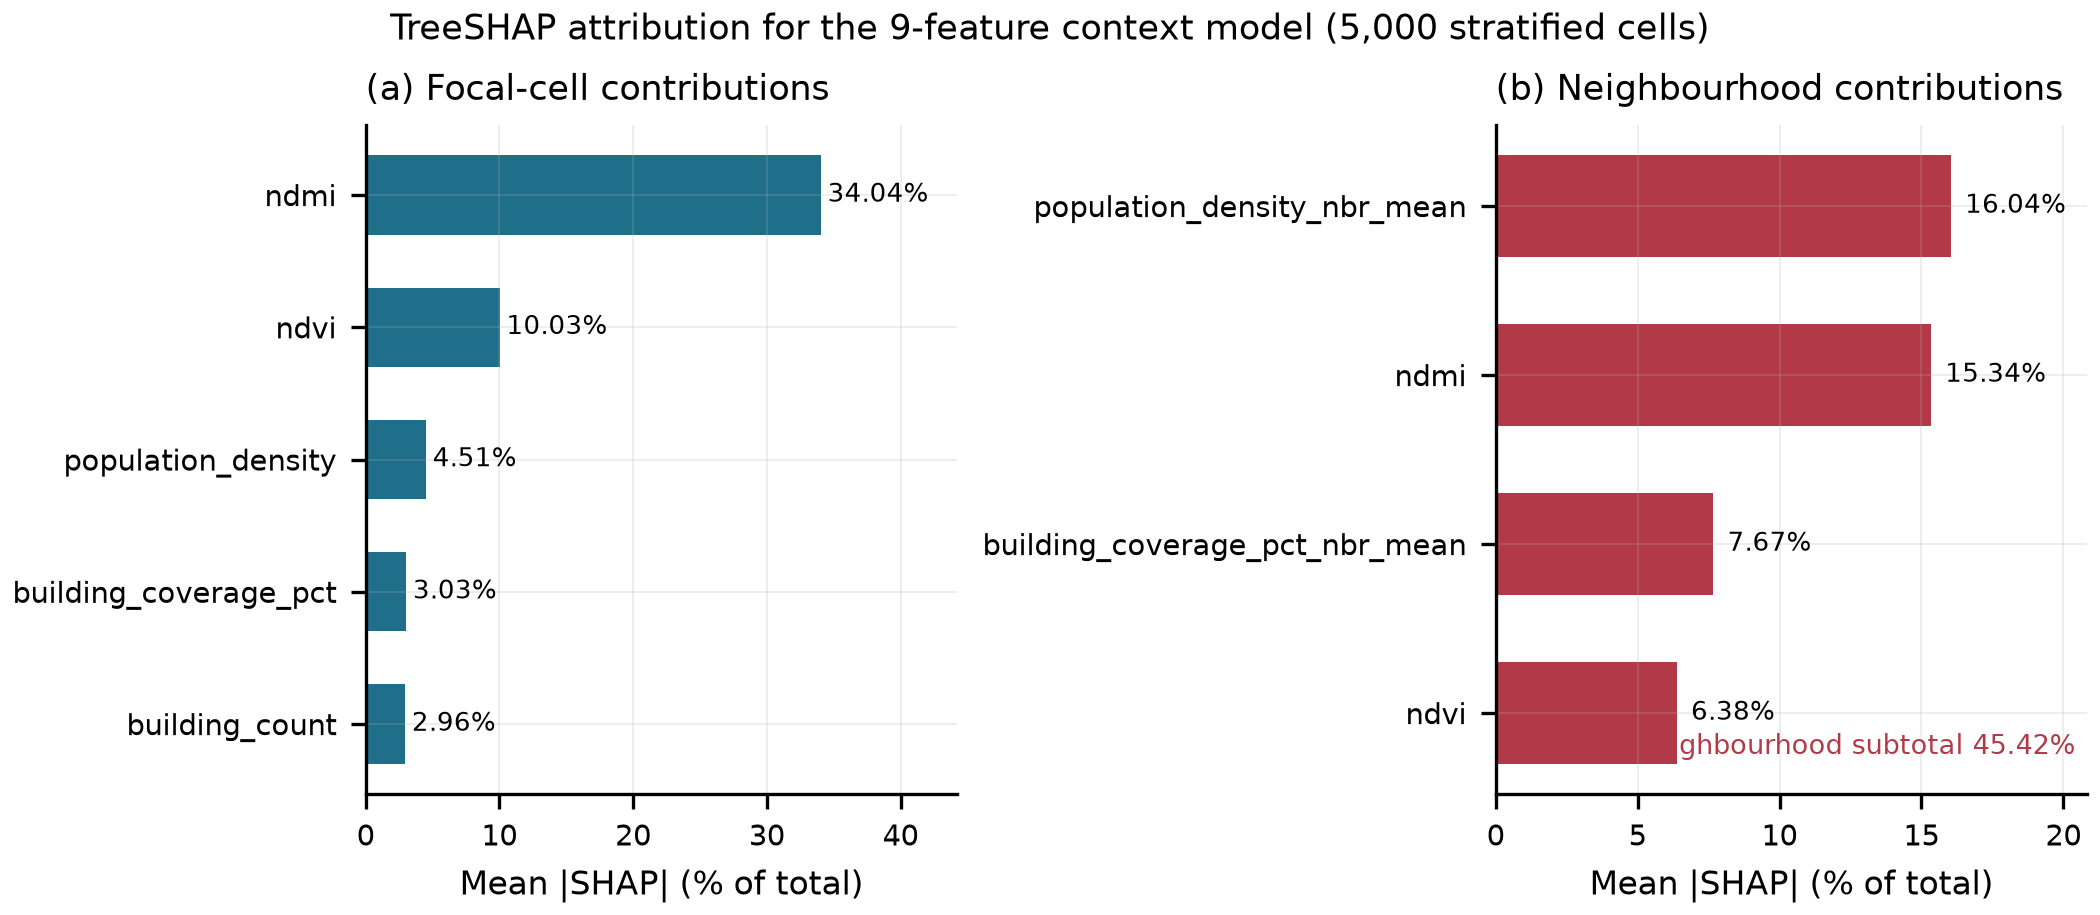
\includegraphics[width=\linewidth]{figures/fig4_shap.png}
\caption{TreeSHAP global attribution for the context model, split into focal-cell and neighbourhood contributions. Attributions are associational model decompositions, not causal effects.}
\label{fig:4}
\end{figure*}


We also report an additivity diagnostic, since the explainer uses interventional perturbation
estimated from a 100-row background sample and therefore satisfies additivity only approximately. The
absolute discrepancy between \(\mathrm{base} + \sum_j \phi_j\) and the model prediction has median
\(1.5 \times 10^{-8}\) \textdegree{}C and mean \(4.6 \times 10^{-4}\) \textdegree{}C, but a maximum of 1.09 \textdegree{}C; 19 of 5,000
evaluated cells (0.38\%) exceed 0.01 \textdegree{}C. For the worst affected cell this residual is comparable to a
full model error, so we report the distribution rather than a summary statistic alone.

\begin{figure*}[!t]
\centering
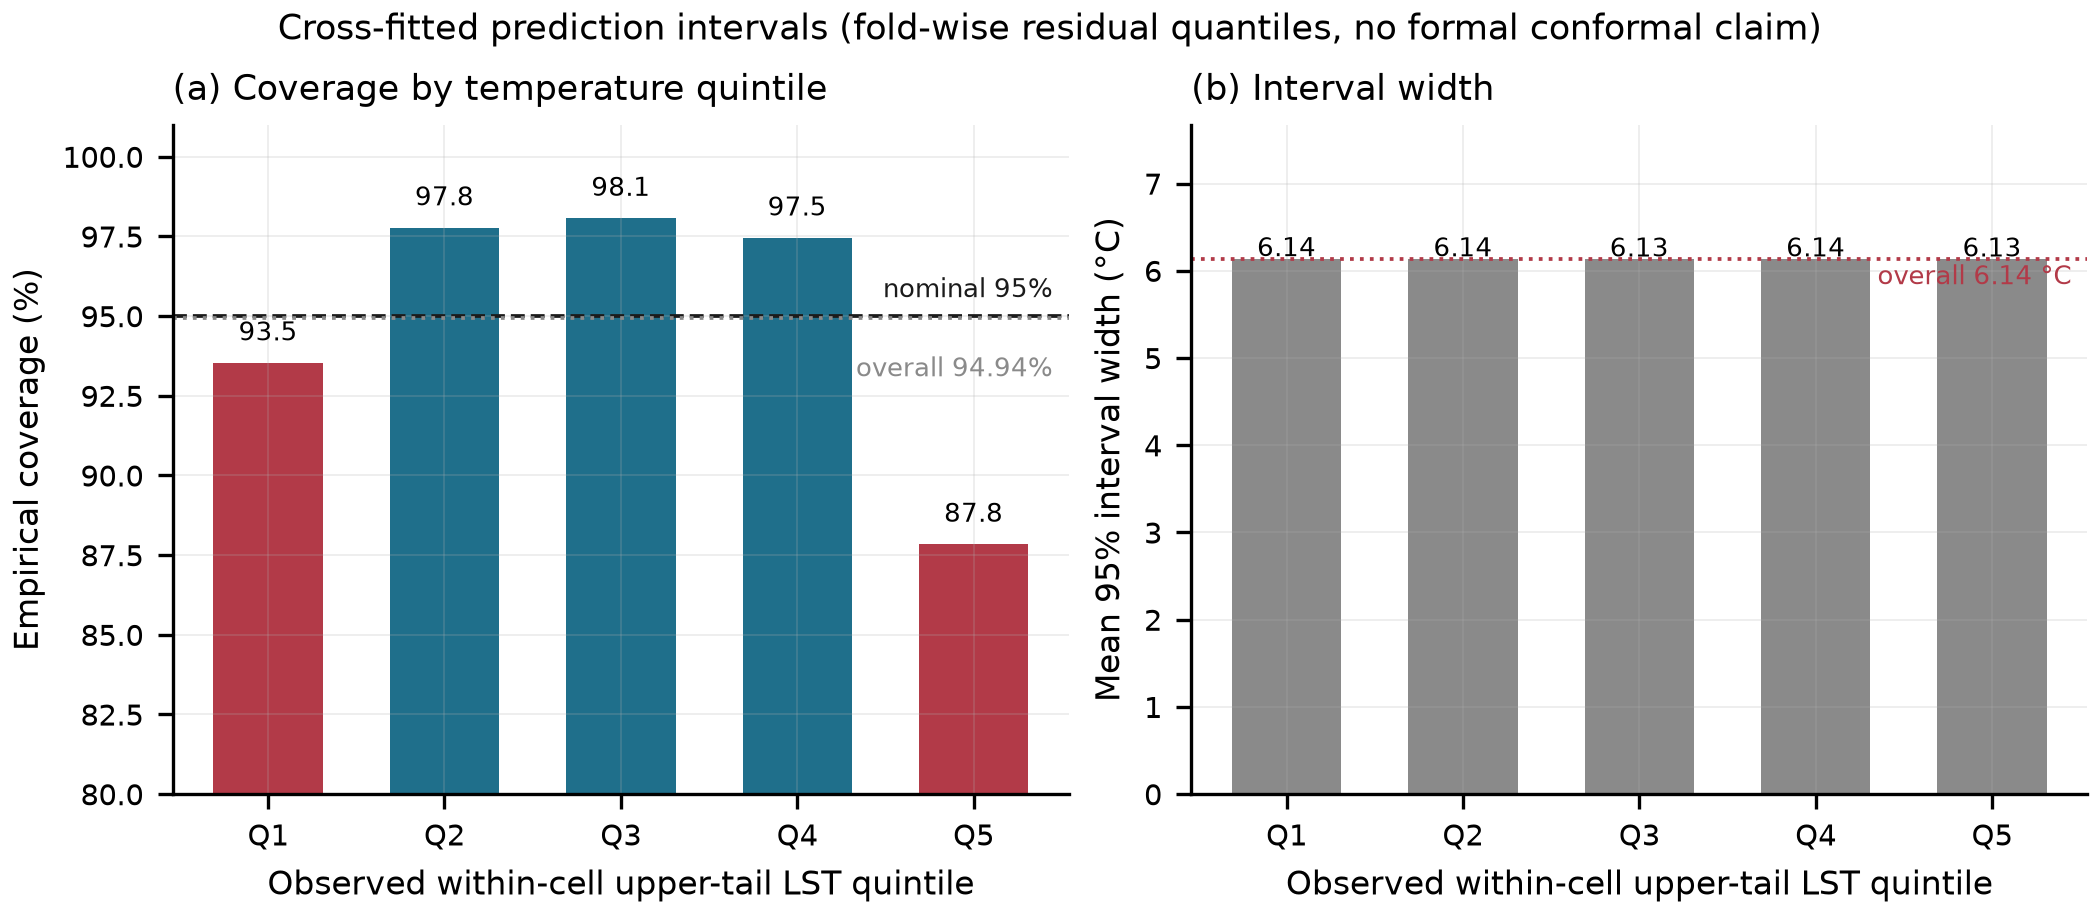
\includegraphics[width=\linewidth]{figures/fig5_uncertainty.png}
\caption{Cross-fitted 95\% prediction intervals: empirical coverage and width by observed temperature quintile. Overall coverage is 94.94\%.}
\label{fig:5}
\end{figure*}


\subsection{Predictive uncertainty}\label{d.-predictive-uncertainty}

Cross-fitted intervals achieve \textbf{94.94\%} overall coverage at a mean width of \textbf{6.14 \textdegree{}C} (Table IV).
Width is effectively constant across quintiles (6.134--6.138 \textdegree{}C), which is a direct consequence of the
symmetric, quantile-based construction: it cannot adapt to heteroscedasticity. The consequence is
visible in coverage, which ranges from 98.07\% in the third quintile to \textbf{87.85\% in the hottest
quintile}. The pooled number is therefore close to nominal for a reason that does not hold in the
part of the distribution that matters most: the model is over-confident where it is warmest, and the
residual bias documented in Section VI-C is the direct cause. A heteroscedastic scheme was also
implemented, but its calibration factor is estimated on the same cells whose coverage it then
reports, so its 95.00\% coverage is close to definitional and its half-widths are roughly 2.5 times the
model's typical error; we do not present it as validated. It is retained in the codebase only as a
relative risk-ranking layer, which is the sole use the priority construction makes of it.

\begin{table}[!t]
\caption{Cross-fitted 95\% prediction intervals (21,815 cells).}
\label{tab:4}
\centering
\footnotesize
\begin{tabular}{@{}llll@{}}
\toprule\noalign{}
Group & Cells & Coverage (\%) & Mean width (\textdegree{}C) \\
\midrule\noalign{}
All & 21,815 & 94.94 & 6.136 \\
Q1 (coolest) & 4,364 & 93.54 & 6.138 \\
Q2 & 4,362 & 97.78 & 6.136 \\
Q3 & 4,363 & 98.07 & 6.134 \\
Q4 & 4,365 & 97.46 & 6.135 \\
Q5 (hottest) & 4,361 & \textbf{87.85} & 6.134 \\
\end{tabular}
\end{table}


\subsection{Equity-constrained allocation}\label{e.-equity-constrained-allocation}

\begin{table}[!t]
\caption{Scenario parameters (dimensionless index units).}
\label{tab:5}
\centering
\footnotesize
\begin{tabular}{@{}llll@{}}
\toprule\noalign{}
Intervention & Unit cost & Effect coefficient & Capacity (cells) \\
\midrule\noalign{}
Urban tree & 1.0 & 1.0 & 1,000 \\
Shade structure & 1.4 & 1.2 & 1,500 \\
Cool roof & 2.0 & 1.1 & 800 \\
Cooling centre & 2.5 & 1.3 & 800 \\
\end{tabular}
\end{table}


The equity-priority set \(\mathcal{E}\) comprises the top 30\% of cells by structural vulnerability. As
Section III-G notes, structural vulnerability is a monotone function of log population density scaled
by built-form capacity, so \(\mathcal{E}\) is effectively a high-density set. The equity constraint (9)
is consequently a \emph{density-weighted benefit-share floor} and should be read as such.

\textbf{E.1 Capacity-bound configuration.} With per-type capacities binding and the budget slack at 35.6\%
utilisation, the mixed-integer optimum selects 4,100 cells --- every capacity ceiling exactly --- for a
total benefit of 2074.49. A benefit-per-cost greedy selects 3,629 cells for a benefit of 1616.44, an
apparent 28.34\% gap. We report this number with its mechanism attached: it is a capacity-saturation
result, not a budget-efficiency result. The optimiser gains because it is free to fill every ceiling,
whereas greedy stops when no further item fits its ratio ordering. An equity floor of
\(\alpha = 0.6\) leaves the solution \emph{unchanged}, because the unconstrained optimum already delivers a
62.16\% equity share; the row is identical to the unconstrained row and carries no information. Only
\(\alpha = 0.7\) binds, reducing benefit to 1996.90, a 3.74\% cost.

\textbf{E.2 Budget-bound configuration.} Setting the budget to \(f\) times the cost of filling every capacity
makes the budget the active constraint. Total benefit rises from 859.57 at \(f = 0.25\) to 2074.49 at
\(f = 1.0\), while the equity share falls from 94.0\% to 62.2\% --- a genuine and interpretable trade-off in
which scarce budget is disproportionately absorbed by cells outside the equity set. Equity floors at or
below 0.6 are inert at every budget level (the solution is unchanged), so only \(\alpha = 0.7\) and 0.8
produce distinct allocations; at \(f = 0.75\), \(\alpha = 0.8\) forces benefit down to 1750.75.

\begin{table*}[!t]
\caption{Allocation results. Costs and benefits are dimensionless scenario units.}
\label{tab:6}
\centering
\footnotesize
\begin{tabular}{@{}
>{\raggedright\arraybackslash}p{(\linewidth - 12\tabcolsep) * \real{0.1429}}
  >{\raggedright\arraybackslash}p{(\linewidth - 12\tabcolsep) * \real{0.1429}}
  >{\raggedright\arraybackslash}p{(\linewidth - 12\tabcolsep) * \real{0.1429}}
  >{\raggedright\arraybackslash}p{(\linewidth - 12\tabcolsep) * \real{0.1429}}
  >{\raggedright\arraybackslash}p{(\linewidth - 12\tabcolsep) * \real{0.1429}}
  >{\raggedright\arraybackslash}p{(\linewidth - 12\tabcolsep) * \real{0.1429}}
  >{\raggedright\arraybackslash}p{(\linewidth - 12\tabcolsep) * \real{0.1429}}@{}}
\toprule\noalign{}
\begin{minipage}[b]{\linewidth}\raggedright
Configuration
\end{minipage} & \begin{minipage}[b]{\linewidth}\raggedright
Constraint active
\end{minipage} & \begin{minipage}[b]{\linewidth}\raggedright
Equity floor
\end{minipage} & \begin{minipage}[b]{\linewidth}\raggedright
Cells
\end{minipage} & \begin{minipage}[b]{\linewidth}\raggedright
Cost
\end{minipage} & \begin{minipage}[b]{\linewidth}\raggedright
Benefit
\end{minipage} & \begin{minipage}[b]{\linewidth}\raggedright
Equity share
\end{minipage} \\
\midrule\noalign{}
Capacity-bound & Capacity (budget 35.6\% used) & --- & 4,100 & 6,700 & 2074.49 & 0.6216 \\
Capacity-bound & Capacity & 0.60 & 4,100 & 6,700 & 2074.49 & 0.6216 (inactive) \\
Capacity-bound & Capacity & 0.70 & 4,100 & 6,700 & 1996.90 & 0.7000 \\
Budget-bound & Budget (\(f\) = 0.25) & --- & 1,482 & 1,674.8 & 859.57 & 0.9401 \\
Budget-bound & Budget (\(f\) = 0.50) & --- & 2,609 & 3,350 & 1502.00 & 0.8233 \\
Budget-bound & Budget (\(f\) = 0.75) & --- & 3,287 & 5,024.5 & 1874.02 & 0.7250 \\
Budget-bound & Budget (\(f\) = 1.00) & --- & 4,100 & 6,700 & 2074.49 & 0.6216 \\
Budget-bound & Budget (\(f\) = 0.75) & 0.80 & 3,147 & 5,024.0 & 1750.75 & 0.8000 \\
\end{tabular}
\end{table*}


A second configuration, in which the budget is defined as a fraction of mean per-cell cost and no
capacity limits apply, yields the clearest measure of what the equity constraint costs. Its
unconstrained optimum (benefit 2470.69, equity share 0.5687) is reproduced exactly by a simple
ranking baseline, which independently confirms optimality. Imposing floors then gives: \(\alpha = 0.5\)
no change; \(\alpha = 0.6\) benefit 2341.74 (\textbf{\textminus{}5.22\%}); \(\alpha = 0.7\) benefit 2007.31 (\textbf{\textminus{}18.76\%}),
with the equity share pinned at the target in each case and solver status optimal with relative MIP
gap below \(8 \times 10^{-5}\). \textbf{Requiring that 70\% of benefit accrue to equity-priority cells costs
18.76\% of total benefit; a 60\% floor costs 5.22\%.}

\textbf{E.3 What the effect coefficients can and cannot do.} Because \(\mathrm{effect}_t\) is
cell-invariant in (4), it cannot change which intervention is preferred at any cell, nor any
per-cell ranking of cells. We verified this directly: multiplying all effect coefficients by a common
scalar leaves every allocation decision unchanged. We therefore make no claim about the relative
effectiveness of the four intervention types. Their only influence is through the cost--benefit
trade-off, where a higher effect and a higher cost together determine which types a tight budget
favours --- an assumption we state rather than a result we estimate.

\begin{figure*}[!t]
\centering
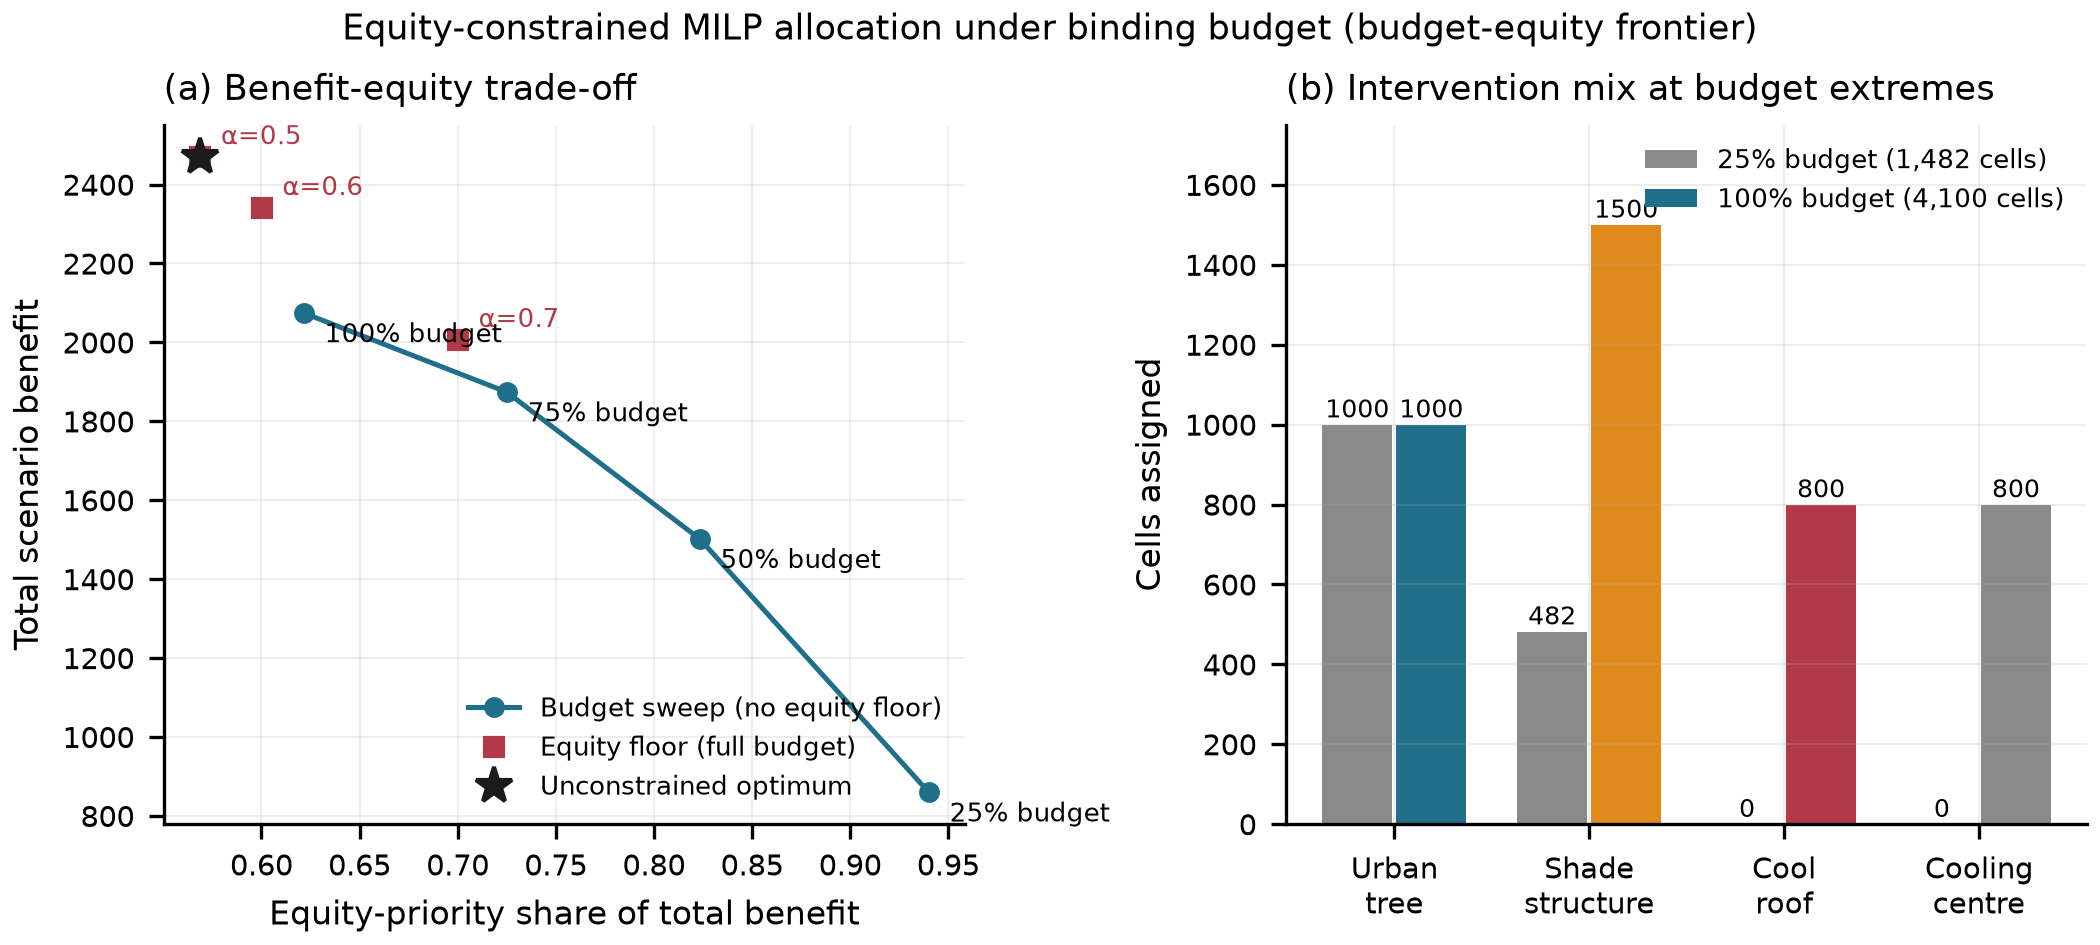
\includegraphics[width=\linewidth]{figures/fig6_optimization.png}
\caption{Allocation panels: (a) benefit--equity trade-off for the budget sweep and the equity floors, and (b) intervention mix at the budget extremes, where the 25\% budget is absorbed almost entirely by urban trees while the full budget saturates all four types.}
\label{fig:6}
\end{figure*}


\subsection{Eligibility}\label{f.-eligibility}

5,084 of 21,815 cells (23.3\%) are eligible for at least one intervention: 4,192 for urban trees, 3,274
for cool roofs, 2,925 for shade structures and 2,520 for cooling centres. This rate should not be
read as an empirical finding about Bengaluru. Every gate is a conjunction of in-sample median and
quartile thresholds, so 23.3\% is close to what the threshold definitions imply rather than a
property of the city. Externally justified thresholds --- canopy targets or planning standards --- would
be required to make the number informative.

\subsection{Robustness}\label{g.-robustness}

Of 500 Monte Carlo runs, 475 return a certified-optimal solution and 25 terminate on the 20-second
time limit, which is recorded as a missing value rather than as a failure flag. All 192
certified-optimal equity runs satisfy their equity target; the 8 time-limited equity runs cannot be
assessed. Each run perturbs cost and effect by up to \textpm{}30\% and capacities by up to \textpm{}20\%. The 500 runs
share 150 distinct parameter draws, each evaluated across several budget and equity settings, so the
budget and equity levels are not independent replications.

\section{Discussion}\label{vii.-discussion}

Three results carry practical significance.

\textbf{Neighbourhood context is worth more for error balance than for accuracy.} A 3.62\% RMSE reduction is
a modest gain that a practitioner might reasonably dismiss. The 8.08\% reduction in hottest-quintile
bias is a different kind of result, because the hottest quintile is where an adaptation budget should
be concentrated and where the model was demonstrably least trustworthy.

\textbf{Pooled uncertainty metrics conceal the failure mode that matters.} Reporting 94.94\% coverage would
be accurate and uninformative. The 87.85\% figure in the hottest quintile, paired with a constant
interval width, identifies a specific, actionable weakness: the interval construction is symmetric
and cannot widen where the model is over-confident. A municipality relying on these intervals to
trigger intervention would find the trigger firing too late in exactly the neighbourhoods where
heat is most dangerous. We regard the per-quintile breakdown as a reporting requirement for any
spatial prediction interval, not an optional diagnostic.

\textbf{Equity has a measurable price, and the price depends on how binding the constraint is.} A 60\%
equity floor costs 5.22\% of benefit; a 70\% floor costs 18.76\%. Meanwhile budgets below full capacity
deliver \emph{higher} equity shares for free in benefit terms --- the \(f = 0.25\) solution is 94.0\% equitable,
because scarce budget is absorbed disproportionately outside the equity set. For a municipality
operating under severe fiscal constraint, this is the practically important finding: tightening the
budget is itself an equity measure, and a formal equity constraint on top of a tight budget mostly
redistributes allocation rather than increasing total benefit.

Two negative results deserve equal visibility. First, the effect coefficients cannot influence
allocation preference (Section VI-E.3); any study that reports intervention-type preferences derived
from cell-invariant coefficients is reporting its own opportunity weights back to itself. Second,
the NDBI/NDMI identity (Section VI-B) means index-based UHI studies that include both are
double-counting a single axis, which may contribute to the persistent difficulty in separating
built-form from vegetation effects.

\section{Limitations}\label{viii.-limitations}

We enumerate limitations that materially constrain interpretation, separating those that changed how
results are framed from those that remain open.

\textbf{L1 --- Single-date spatial percentile, not a temporal extreme.} The target is the 95th percentile of
valid 30 m pixels \emph{within one 250 m cell on one acquisition}. It is not a daily maximum, a heatwave
intensity, or a climatological extreme, and no temporal stack exists in the implementation. Every
result in this paper is conditional on that definition. A multi-date hot-season composite is the single
most important extension and would change all reported numbers.

\textbf{L2 --- Surface temperature is not air temperature.} LST is a validated but imperfect proxy for human
thermal exposure {[}3{]}--{[}5{]}, {[}11{]}, and the divergence depends on time of day, season and surface
moisture. HeatScope does not estimate air temperature, thermal comfort, or any health outcome.

\textbf{L3 --- Systematic under-prediction of the hottest cells.} A +1.38 \textdegree{}C bias in the hottest quintile
survives at 8.08\% reduction with added context features. Because this bias coincides with the
under-coverage reported in Section VI-D, it is the most consequential empirical weakness in the
pipeline, and it biases exposure estimates downward precisely where they matter most.

\textbf{L4 --- Intervals lack a coverage guarantee.} Quantiles are estimated by linear interpolation rather
than the conformal index, and calibration residuals for a fold originate from models trained on folds
including it {[}30{]}, {[}31{]}. The reported 94.94\% is an empirical measurement on this dataset, not a
guarantee for future data.

\textbf{L5 --- Equity is population density.} The equity set is a monotone function of log population
density scaled by built-form capacity. A genuine equity criterion would require health, demographic
or socioeconomic layers the study does not contain.

\textbf{L6 --- Eligibility rates are definitional.} The 23.3\% eligibility rate follows from in-sample
quantile gates and is not an empirical property of the city.

\textbf{L7 --- Scenario parameters are assumptions.} Costs, effect coefficients and capacities are
dimensionless index units with no empirical calibration. Benefit totals and cost-of-equity figures
are internal to this scenario and must not be read as degrees, currency, or health outcomes.

\textbf{L8 --- Vulnerability index weights are unjustified.} The exposure and capacity weights are
expert-elicited, untested, and combined multiplicatively, which collapses cells that are simultaneously
low-vegetation, low-population and high-built toward zero before a second rescaling. The sensitivity
component is a single variable. We report the index as one descriptive layer, not a validated
construct.

\textbf{L9 --- Study region and resolution.} The region is a bounding box rather than an administrative
boundary; 30 boundary cells have area as small as 10.54 m², and their p95 target derives from
approximately one source pixel. Equity findings are known to be sensitive to analysis scale {[}35{]}.

\textbf{L10 --- Data provenance gaps.} The population raster has no recorded release DOI, licence or
checksum, and is aggregated without proportional-area weighting. The building layer comes from a
single quadkey tile of a 2026-08-13 conflation snapshot with no in-repository downloader, no
de-duplication of overlapping footprints, no minimum-area gate on boundary slivers, and its available
\texttt{height} attribute is discarded.

\textbf{L11 --- Reproducibility gaps.} Acquisition is not idempotent: the search window derives from the
current date and the lowest-cloud scene is selected, so re-running selects a different scene and
silently invalidates all downstream artifacts. The declared dependency set omits scikit-learn, SHAP,
SciPy, XGBoost and the STAC clients, and XGBoost is imported defensively so its benchmark row depends
on an undeclared environment. No hardware, runtime or memory metadata is recorded. The public
repository excludes all data and result directories.

\textbf{L12 --- Solver robustness.} 25 of 500 sensitivity runs hit the time limit and are recorded as
missing values; no MIP gap is passed in that experiment. Equity targets at or below 0.6 are inert in
both reported configurations.

\textbf{L13 --- No verified prior formulation.} We could not verify a peer-reviewed mixed-integer or linear
programme allocating urban heat mitigation under equity constraints. The novelty claim is therefore
stated as ``no directly comparable framework was identified in the literature we verified'' rather than
as an absolute priority claim.

\textbf{L14 --- Single region, single date.} All results are for one bounding box on one acquisition date.
Transfer to other cities, other seasons, or other dates is untested, and the region cannot be shown to
represent Bengaluru's administrative area.

\section{Conclusion}\label{ix.-conclusion}

We presented HeatScope, an auditable pipeline for urban heat exposure mapping and mitigation
prioritisation at 250 m resolution for Bengaluru, and we reported its results together with the
findings that constrain how they may be used. Spatially structured validation across 240 blocks, a
3.62\% RMSE improvement from neighbourhood context, 94.94\% empirical interval coverage with an
exposed 87.85\% coverage deficit in the hottest quintile, and an equity-constrained allocation in which
a 70\% benefit-share floor costs 18.76\% of benefit, together constitute the empirical contribution.

The negative results are equally part of that contribution. We established that a widely used pair of
spectral indices is algebraically redundant; that cell-invariant effect coefficients cannot influence
allocation preference; that pooled coverage metrics conceal a systematic failure in the hottest
quintile; and that six claims one might reasonably have expected to hold --- heatwave intensity,
causal attribution, air-temperature prediction, conformal coverage, physical benefit units, and
methodological novelty --- do not hold for this system and are reported here as such.

Priority for future work follows directly: build a multi-date hot-season composite so that the target
is a temporal statistic; obtain the socioeconomic layers required for an equity criterion that is not
a restatement of population density; replace the symmetric interval construction with a
heteroscedastic, split-disjoint scheme that can widen where the model is over-confident; and calibrate
cost, effect and capacity parameters against observed outcomes so that the allocation stage produces
quantities with physical units. Code, intermediate artifacts, and the full audit trail accompanying
this paper are available at the project repository.

\section{Acknowledgment}\label{acknowledgment}

The author thanks the maintainers of the Landsat, WorldPop and Overture Maps programmes for open
access to the data products used in this work.

\begin{thebibliography}{99}
\bibitem{ref1} U.S. Geological Survey, ``How do I use a scale factor for Landsat Level-2 science products?''
Landsat Collection 2 FAQ, U.S. Department of the Interior. {[}Online{]}. Available:
https://www.usgs.gov/faqs/how-do-i-use-a-scale-factor-landsat-level-2-science-products


\bibitem{ref2} U.S. Geological Survey EROS, ``Landsat Collection 2 surface temperature.'' {[}Online{]}. Available:
https://www.usgs.gov/landsat-missions/landsat-collection-2-surface-temperature


\bibitem{ref3} X. Meng, J. Cheng, B. Yao, and Y. Guo, ``Validation of the ECOSTRESS land surface temperature
product using ground measurements,'' \emph{IEEE Geosci. Remote Sens. Lett.}, vol.~19, pp.~1--5, 2022.


\bibitem{ref4} S. Li, J. Wang, D. Li, Z. Ran, and B. Yang, ``Evaluation of Landsat 8-like land surface temperature
by fusing Landsat 8 and MODIS land surface temperature product,'' \emph{Processes}, vol.~9, no. 12,
art. 2262, 2021.


\bibitem{ref5} J. A. Voogt and T. R. Oke, ``Thermal remote sensing of urban climates,'' \emph{Remote Sens. Environ.},
vol.~86, no. 3, pp.~370--384, 2003.


\bibitem{ref6} D. Zhou et al., ``Satellite remote sensing of surface urban heat islands: progress, challenges, and
perspectives,'' \emph{Remote Sens.}, vol.~11, no. 1, art. 48, 2019.


\bibitem{ref7} C. R. Almeida, A. C. Teodoro, and A. Gonçalves, ``Study of the urban heat island (UHI) using remote
sensing data/techniques: a systematic review,'' \emph{Environments}, vol.~8, no. 10, art. 105, 2021.


\bibitem{ref8} M. Santamouris, ``Recent progress on urban overheating and heat island research. Integrated
assessment of the energy, environmental, vulnerability and health impact,'' \emph{Energy Build.}, vol.~207,
art. 109482, 2020.


\bibitem{ref9} K. Deilami, M. Kamruzzaman, and Q. Liu, ``Urban heat island effect: a systematic review of
spatio-temporal factors, data, methods, and mitigation measures,'' \emph{Int. J. Appl. Earth Obs.
Geoinf.}, vol.~67, pp.~30--42, 2018.


\bibitem{ref10} G. Manoli et al., ``Magnitude of urban heat islands largely explained by climate and population,''
\emph{Nature}, vol.~573, no. 7772, pp.~55--60, 2019.


\bibitem{ref11} C. Heaviside, H. Macintyre, and S. Vardoulakis, ``The urban heat island: implications for health in
a changing environment,'' \emph{Curr. Environ. Health Rep.}, vol.~4, no. 3, pp.~296--305, 2017.


\bibitem{ref12} E. L. Kruger, C. A. Tamura, P. Bröde, M. Schweiker, and A. Wagner, ``Short- and long-term
acclimatization in outdoor spaces: exposure time, seasonal and heatwave adaptation effects,'' \emph{Build.
Environ.}, vol.~116, pp.~17--29, 2017.


\bibitem{ref13} N. Mondal and P. Anand, ``Influence of urbanization on heat exposure risk across Indian cities,''
\emph{Sustain. Cities Soc.}, vol.~135, art. 106960, 2025.


\bibitem{ref14} A. Hsu, G. Sheriff, T. Chakraborty, and D. Manya, ``Disproportionate exposure to urban heat island
intensity across major US cities,'' \emph{Nat. Commun.}, vol.~12, no. 1, art. 2721, 2021.


\bibitem{ref15} B.-C. Gao, ``NDWI --- A normalized difference water index for remote sensing of vegetation liquid
water from space,'' \emph{Remote Sens. Environ.}, vol.~58, no. 3, pp.~257--266, 1996.


\bibitem{ref16} Y. Zha, J. Gao, and S. Ni, ``Use of normalized difference built-up index in automatically mapping
urban areas from TM imagery,'' \emph{Int. J. Remote Sens.}, vol.~24, no. 3, pp.~583--594, 2003.


\bibitem{ref17} J. W. Rouse, S. N. Goward, and V. I. V, ``Vegetation in sensor space,'' \emph{Remote Sens. Environ.},
vol.~3, pp.~295--309, 1974.


\bibitem{ref18} C. T. Lloyd, A. Sorichetta, and A. J. Tatem, ``High resolution global gridded data for use in
population studies,'' \emph{Sci. Data}, vol.~4, art. 170001, 2017.


\bibitem{ref19} F. R. Stevens, A. E. Gaughan, C. Linard, and A. J. Tatem, ``Disaggregating census data for
population mapping using remotely-sensed and ancillary data,'' \emph{PLoS ONE}, vol.~10, no. 2, e0107042,
2015.


\bibitem{ref20} WorldPop, University of Southampton, ``WorldPop global high resolution population denominators
project (100m),'' doi: 10.5258/SOTON/WP00107.


\bibitem{ref21} Overture Maps Foundation, ``Buildings theme,'' \emph{Overture Maps documentation}, release snapshot
2026-08-13, ODbL. {[}Online{]}. Available: https://docs.overturemaps.org/


\bibitem{ref22} J. H. Friedman, ``Greedy function approximation: a gradient boosting machine,'' \emph{Ann. Stat.},
vol.~29, no. 5, pp.~1189--1231, 2001.


\bibitem{ref23} T. Chen and C. Guestrin, ``XGBoost: a scalable tree boosting system,'' in \emph{Proc. 22nd ACM SIGKDD
Int. Conf. Knowl. Discov. Data Mining}, 2016, pp.~785--794.


\bibitem{ref24} P. Geurts, D. Ernst, and L. Wehenkel, ``Extremely randomized trees,'' \emph{Mach. Learn.}, vol.~63,
no. 1, pp.~3--42, 2006.


\bibitem{ref25} L. Breiman, ``Random forests,'' \emph{Mach. Learn.}, vol.~45, no. 1, pp.~5--32, 2001.


\bibitem{ref26} D. R. Roberts et al., ``Cross-validation strategies for data with temporal, spatial, hierarchical,
or phylogenetic structure,'' \emph{Ecography}, vol.~40, no. 8, pp.~913--929, 2017.


\bibitem{ref27} P. Ploton et al., ``Spatial validation reveals poor predictive performance of large-scale ecological
mapping models,'' \emph{Nat. Commun.}, vol.~11, no. 1, art. 4540, 2020.


\bibitem{ref28} S. M. Lundberg, G. Erion, H. Chen, A. DeGrave, J. M. Prutkin, B. Nair, R. Katz, J. Himmelfarb,
N. Bansal, and S.-I. Lee, ``From local explanations to global understanding with explainable AI for
trees,'' \emph{Nat. Mach. Intell.}, vol.~2, no. 1, pp.~56--67, 2020.


\bibitem{ref29} S. M. Lundberg and S.-I. Lee, ``A unified approach to interpreting model predictions,'' in \emph{Adv.
Neural Inf. Process. Syst.}, vol.~30, 2017.


\bibitem{ref30} J. Lei, M. J. G'Sell, A. Rinaldo, R. J. Tibshirani, and L. Wasserman, ``Distribution-free
predictive inference for regression,'' \emph{J. Amer. Stat. Assoc.}, vol.~113, no. 523, pp.~1094--1111, 2018.


\bibitem{ref31} A. N. Angelopoulos and S. Bates, ``Conformal prediction: a gentle introduction,'' \emph{Found. Trends
Mach. Learn.}, vol.~16, no. 4, pp.~494--591, 2023.


\bibitem{ref32} A. Saltelli, K. Aleksankina, W. Becker, P. Fennell, F. Ferretti, N. Holst, S. Li, and Q. Wu, ``Why
so many published sensitivity analyses are false: a systematic review of sensitivity analysis
practices,'' \emph{Environ. Model. Softw.}, vol.~114, pp.~29--39, 2019.


\bibitem{ref33} E. K. Chu and C. E. B. Cannon, ``Equity, inclusion, and justice as criteria for decision-making on
climate adaptation in cities,'' \emph{Curr. Opin. Environ. Sustain.}, vol.~51, pp.~85--94, 2021.


\bibitem{ref34} S. Juhola, M. Heikkinen, T. Pietilä, F. Groundstroem, and J. Käyhkö, ``Connecting climate justice
and adaptation planning: an adaptation justice index,'' \emph{Environ. Sci. Policy}, vol.~136, pp.~609--619,
2022.


\bibitem{ref35} C. Carvalho, A. G. Del Campo, and D. de Carvalho Cabral, ``Scales of inequality: the role of spatial
extent in environmental justice analysis,'' \emph{Landsc. Urban Plan.}, vol.~221, art. 104369, 2022.


\bibitem{ref36} S. Kanga et al., ``Understanding the linkage between urban growth and land surface temperature ---
a case study of Bangalore city, India,'' \emph{Remote Sens.}, vol.~14, no. 17, art. 4241, 2022.


\bibitem{ref37} N. R. Govind and H. Ramesh, ``Exploring the relationship between LST and land cover of Bengaluru by
concentric ring approach,'' \emph{Environ. Monit. Assess.}, vol.~192, no. 10, art. 650, 2020.


\bibitem{ref38} H. Sussman, A. Dai, and P. E. Roundy, ``The controlling factors of urban heat in Bengaluru,
India,'' \emph{Urban Clim.}, vol.~38, art. 100881, 2021.


\bibitem{ref39} A. Mathew, S. Khandelwal, and N. Kaul, ``Investigating spatial and seasonal variations of urban
heat island effect over Jaipur city and its relationship with vegetation, urbanization and elevation
parameters,'' \emph{Sustain. Cities Soc.}, vol.~35, pp.~157--177, 2017.


\bibitem{ref40} Q. Huangfu and J. A. J. Hall, ``Parallelizing the dual revised simplex method,'' \emph{Math. Program.
Comput.}, vol.~10, no. 1, pp.~119--142, 2018.


\bibitem{ref41} Q. Huangfu and J. A. J. Hall, ``HiGHS --- high performance software for linear optimization,'' in
\emph{Proc. 23rd Int. Symp. Math. Program. Theory Oper. Res. (ISMP 2023)}, 2023.
\end{thebibliography}
